% =========================================================================== %
% TeX input file: "download and install scout"
%
% WARNING: this tex file does not compile standalone, it needs to be embedded
% in a master tex document (e.g. ScoutInstallation.tex)
% =========================================================================== %

Before you can install Scout make sure that you have a working Java Development Kit (JDK) installation of version 7 or 8.
To download the Eclipse Scout package visit the official Eclipse download page as shown in \figref{scout_download}.

\begin{figure}
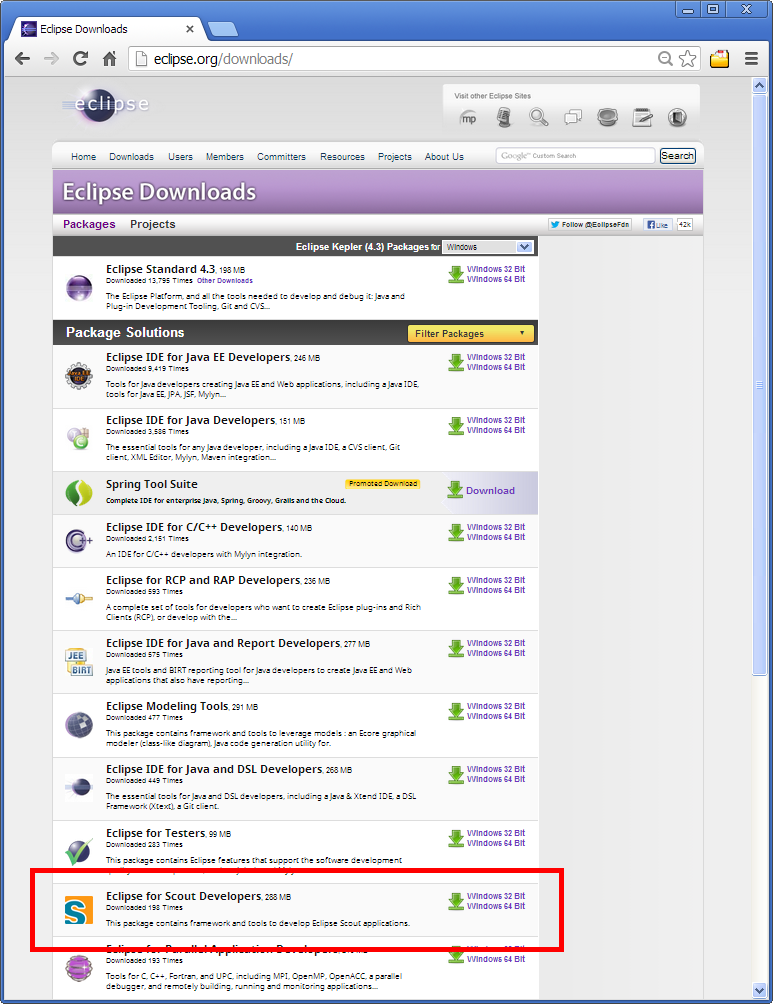
\includegraphics[width=15cm]{scout_download.png}
\caption{The Eclipse download page. The platform filter is set to Windows and the available Packages are filtered for Scout.}
\figlabel{scout_download}
\end{figure}

If the download page shows the wrong platform, manually select the correct platform in the dropdown list.
As shown in \figref{scout_download}, the Scout package is available as a 32 bit and a 46 bit package. 
Make sure to pick the package that matches your JDK installation. 
You can check your installation on the command line as follows.

\begin{lstlisting}[
  language=console
]
console-prompt>java -version
java version "1.7.0_55"
Java(TM) SE Runtime Environment (build 1.7.0_55-b13)
Java HotSpot(TM) 64-Bit Server VM (build 24.55-b03, mixed mode)
\end{lstlisting}

If the output explicitly mentions the 64 bit installation as shown above, you have a 64 bit installation. 
Otherwise, you have a 32 bit JDK installed.
Now you can select the correct Scout package from the Eclipse download site. 
After the package selection, confirm the suggested download mirror as shown in \figref{scout_download_mirror}.

\begin{figure}
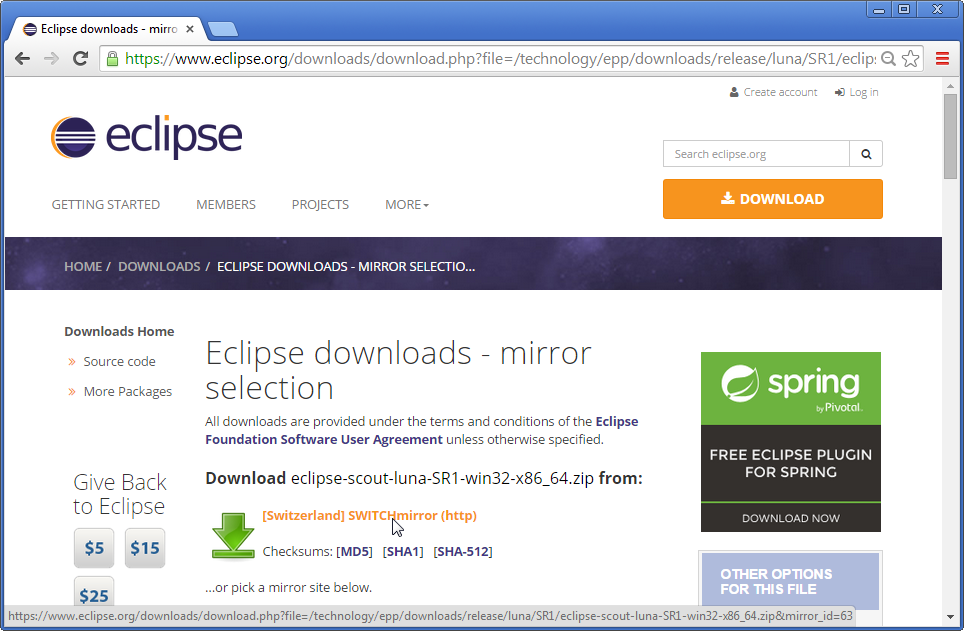
\includegraphics[width=15cm]{scout_download_mirror.png}
\caption{Downloading the Scout package from a mirror.}
\figlabel{scout_download_mirror}
\end{figure}

As the Scout package is a simple ZIP (or tar.gz) file, you may unpack its content to a folder of your choice.
Inside the eclipse sub-folder, you will then find the Eclipse executable file, such as the \texttt{eclipse.exe} file on a Windows plattform. 
Starting the Eclipse executable brings up the workspace launcher as shown in \figref{scout_start}.

\begin{figure}
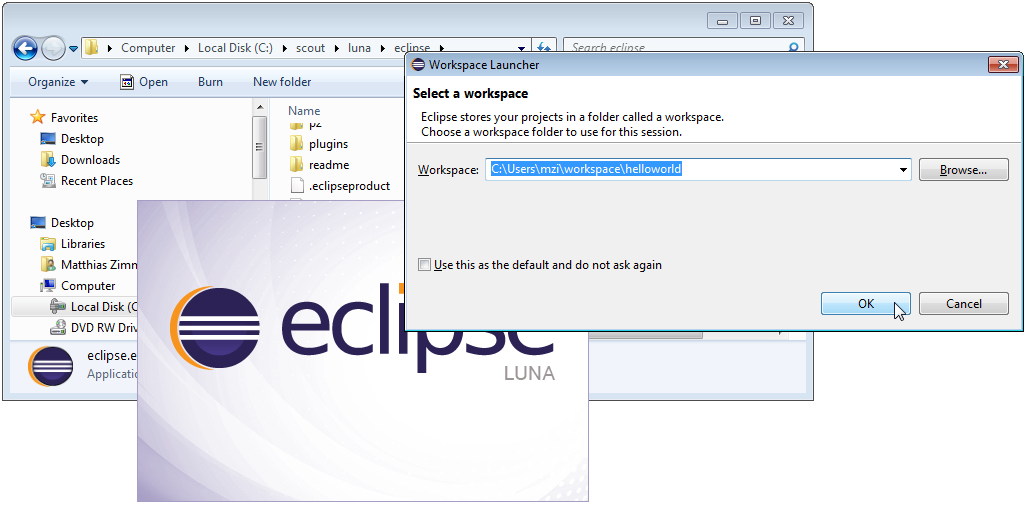
\includegraphics[width=15cm]{scout_startup_select_workspace.png}
\caption{Starting the Eclipse Scout package and selecting an empty workspace.}
\figlabel{scout_start}
\end{figure}

Into the \field{Workspace} you enter an empty target directory for your first Scout project. 
After clicking the \button{Ok}, the Eclipse IDE creates any directories that do not yet exist and opens the specified workspace. 
When opening a new workspace for the first time, Eclipse then displays the welcome screen shown in \figref{scout_welcome}. 

\begin{figure}
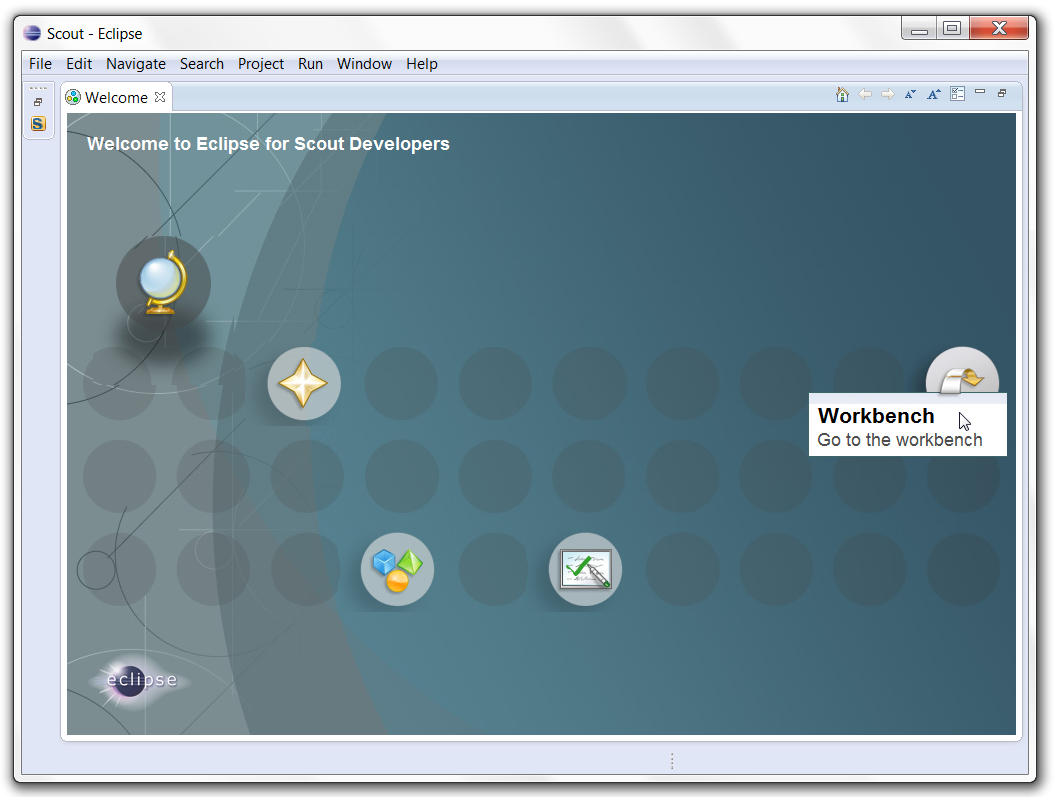
\includegraphics[width=13cm]{scout_startup_welcome.png}
\caption{Eclipse Scout welcome screen.}
\figlabel{scout_welcome}
\end{figure}

To close the welcome page and open the Scout perspective in the Eclipse IDE click on the \icon{Workbench}. 
As a result the empty Scout perspective is displayed according to \figref{scout_perspective}. 

\begin{figure}
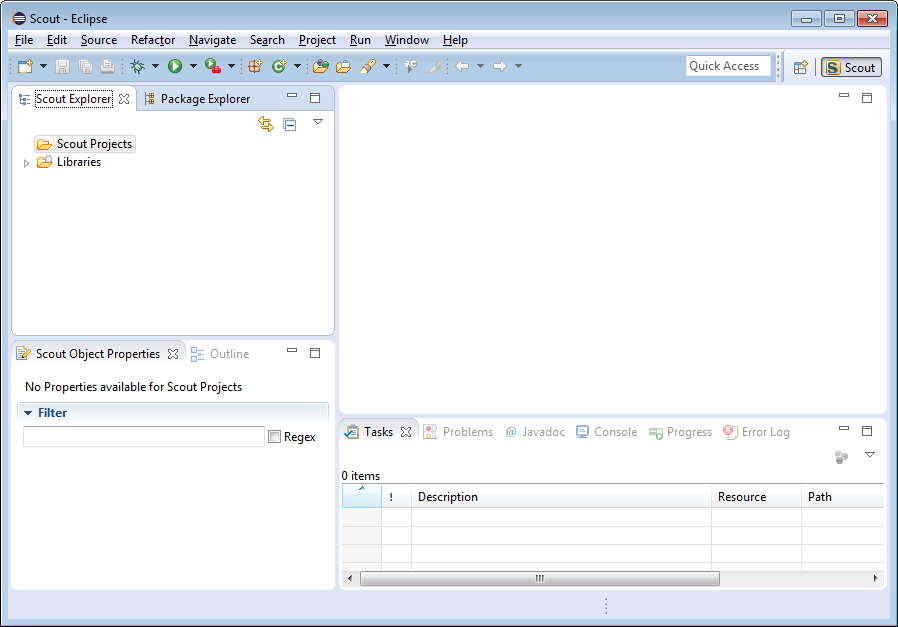
\includegraphics[width=13cm]{scout_startup_scout_explorer.png}
\caption{Eclipse Scout started in the Scout SDK perspective. }
\figlabel{scout_perspective}
\end{figure}

Congratulations, you just have successfully completed the Eclipse Scout installation!

% =========================================================================== %
% EOF TeX input file
% =========================================================================== %
